\chapter{Diseño}

\section{Arquitectura Modelo-Vista-Controlador}

Para facilitar la escalabilidad del sistema se va a seguir el patrón de diseño de arquitectura Modelo-Vista-Controlador (MVC). Esta arquitectura permite un bajo acoplamiento entre los elementos del sistema. Tal y como indica el nombre de la arquitectura, sus componentes principales son tres:

\begin{itemize}
\item Modelo
\item Vista
\item Controlador
\end{itemize}

Teniendo cada uno de los componentes una funcionalidad clara y en gran medida independiente del resto de componentes.

Las principales ventajas de esta arquitectura son las siguientes:

\begin{itemize}
\item Permite la programación paralela e independiente de cada uno de los componentes de la arquitectura.
\item Posibilita la independencia en el funcionamiento de los componentes.
\item Facilita la gestión de errores al ser un sistema modular, dado que los errores estarán más aislados y se podrán abordar de forma más eficiente, y por supuesto también porque se pueden sustituir esos módulos con errores por otros en buen estado.
\item Simplifica la escalabilidad del sistema al poder conectar nuevos módulos de cada uno de los componentes de la arquitectura, sin tener que modificar el resto de componentes.
\item Permite una importante separación entre los datos y su representación visual.
\end{itemize}

Pero todas estas ventajas tienen un coste que hay que asumir, y este coste es principalmente un aumento de complejidad en todos los ámbitos. Por un lado, provoca un aumento de la cantidad de código necesaria, este aumento de código implica tener un mayor número de archivos que mantener; y por último dificulta la curva de aprendizaje del sistema.

A continuación se mostrará una breve definición de cada uno de estos componentes.

\subsection*{Vista}

La Vista es el objeto que maneja la presentación visual de los datos representados por el Modelo, es decir, es la capa sobre la que se muestran los resultados esperados y con la que realiza la interacción el usuario.

\subsection*{Controlador}

El Controlador es el objeto que proporciona significado a las órdenes del usuario, actuando sobre los datos representados por el Modelo. Centra toda la interacción entre la Vista y el Modelo, es decir, es la capa encarga de centralizar todas las conexiones entre el resto de capas, manejando las entradas, transfiriendo las al modelo de forma correcta y devolviendo la respuesta del Modelo a la Vista. Además, es el encargado de modificar el Modelo en caso de que sea necesario.

\subsection*{Modelo}

El Modelo es el objeto que representa la información del programa. Maneja los datos y controla todas sus transformaciones, es decir, contiene y maneja toda la información del sistema, salvo el conocimiento específico del Controlador o de la Vista.

\subsection*{Ciclo de vida de MVC}

Las conexiones entre las distintas partes están muy bien definidas y acotadas para tener un bajo acoplamiento.

El Controlador recibe las entradas del usuario, y transmite las peticiones al Modelo, el cual realiza las tareas de la petición y devuelve el resultado al Controlador; y este a su vez devuelve la respuesta a la Vista para que el usuario pueda observar los resultados de su entrada (Figura \ref{fig:ciclo_vida_MVC}).

\begin{figure}[h]
\centering
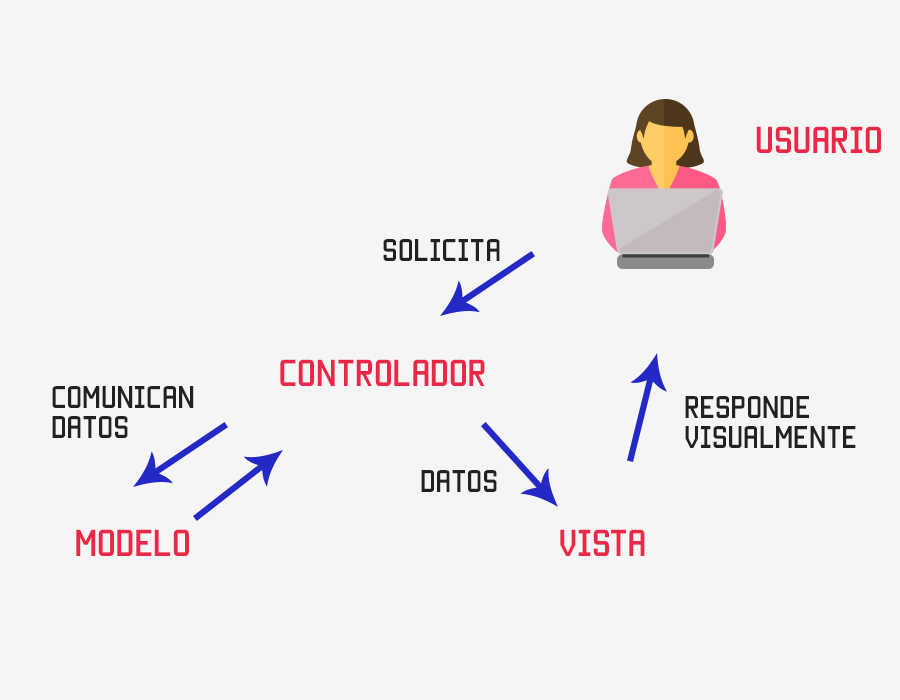
\includegraphics[width=0.8\textwidth]{imagenes/06_Diseno/ciclo_vida_MVC.jpg}
\begin{center}
(Fuente: \url{https://codigofacilito.com/articulos/mvc-model-view-controller-explicado})
\end{center}
\caption{Ciclo de vida de MVC}
\label{fig:ciclo_vida_MVC}
\end{figure}

\section{Diseño de la Vista} \label{sec:diseño_vista}

La Vista de nuestro sistema estará compuesta por el conjunto de páginas web que forman el sitio web donde se permitirá el acceso al chatbot, y por las distintas interfaces de uso del chatbot.

Dado que un objetivo del proyecto es conseguir tener una interfaz sencilla (Tabla \ref{tab:HU2}). Un paso para llegar a este objetivo es el adecuado diseño del movimiento que se puede realizar dentro del sitio web. Una manera sencilla de visualizar este diseño es a través de los sitemaps, que no es más que un esquema visual donde se representan las distintas secciones del sitio web mediante figuras y las conexiones entre estas secciones como flechas que unen las distintas figuras. El sitemap de nuestro sitio web se puede observar en la Figura \ref{fig:sitemap}.

\begin{figure}[h]
\centering
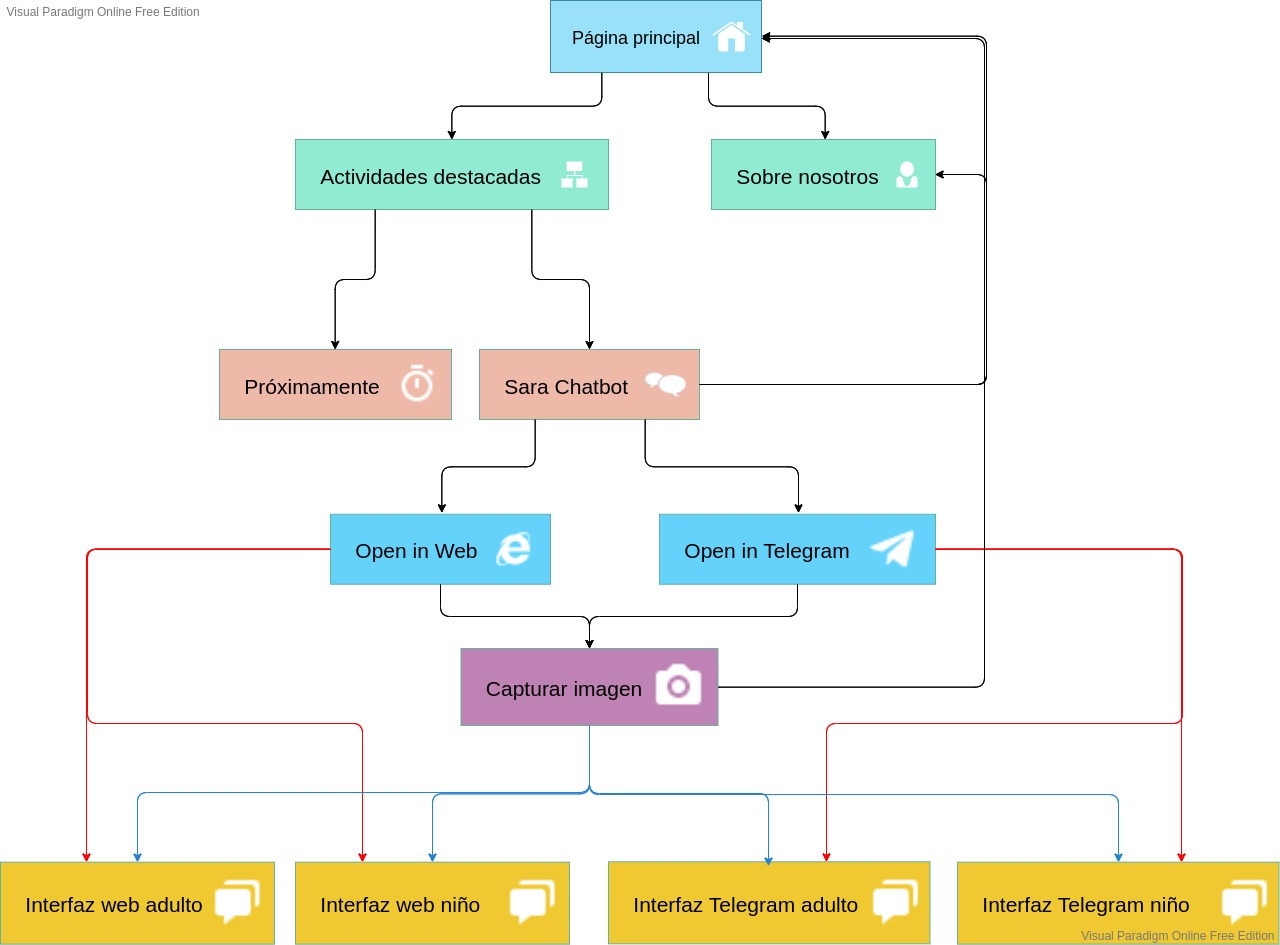
\includegraphics[width=1.1\textwidth]{imagenes/06_Diseno/Sitemap.jpg}
\caption{Sitemap de la Vista}
\label{fig:sitemap}
\end{figure}

Como se puede ver en nuestro sitemap (Figura \ref{fig:sitemap}), el diseño hecho es sencillo, ya que solamente existe una actividad en todo el sitio web, que es la actividad del chatbot. Además, dentro de la actividad mencionada solamente hay dos opciones. Estas opciones deciden el canal por el que se efectuará la conversación con el chatbot. Aunque como se puede apreciar en el sitemap, pasada la elección del canal parece que el diseño se complica, pero en realidad no es así, ya que esta parte del diseño simplemente quiere mostrar como existen dos vías para el acceso a las interfaces con las que hacer uso del chatbot. Estas dos vías se diferencia por un paso, en una de las vías se realiza la captura de imágenes para la deducción de la edad del usuario, mientras que por la otra vía se rechaza esta captura de imágenes y el usuario indica explícitamente su edad, pasando directamente a las interfaces sin tener que pasar por la sección de captura de imágenes. Otra parte a destacar del diseño es la sección de las interfaces, porque como se puede comprobar hay varias secciones de interfaz, incluso varias con el mismo nombre. Esto es debido a que habrá un tipo de interfaz por cada canal disponible para el chatbot, y además dentro de las interfaces de cada canal habrá un tipo de interfaz por cada categoría de edad que exista en el sistema. Por último, cabe destacar que en general en todas las secciones habrá \glspl{link} en la barra de navegación que permitan la vuelta a secciones anteriores para facilitar un movimiento rápido y sencillo por el sitio web.

Otra ayuda para conseguir una interfaz sencilla es el uso de iconos. Estos iconos facilitan la rápida adaptación del usuario al sitio web. Estos iconos permiten la abstracción de cierta información, que de otro debería ser indicada de forma implícita. Para obtener estos iconos se ha hecho uso de páginas web que disponen de conjuntos de iconos gratuitos, recalco lo de gratuitos porque normalmente dentro de estas páginas web existen iconos que son de pago, los cuales pueden tener mayor calidad o mejor diseño. Las principales páginas que se han utilizado son Font Awesome \footnote{\url{https://fontawesome.com/icons}} y Boxicons \footnote{\url{https://boxicons.com/}}. Algunos de los iconos empleados son los mostrados en la Figura \ref{fig:iconos_vista}.

\begin{figure}
\centering
\subfloat[Telegram]{
\label{subfig:telegram_icon}
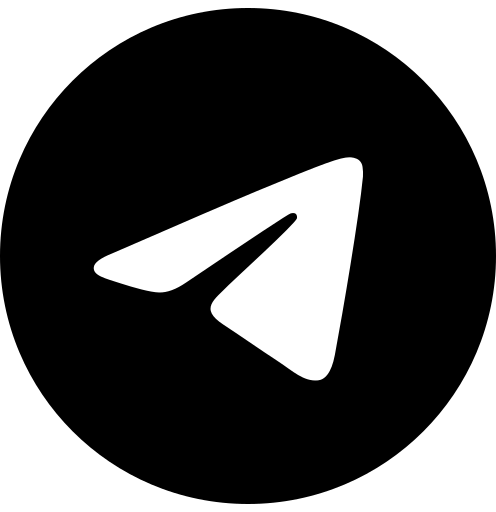
\includegraphics[width=0.2\textwidth]{imagenes/06_Diseno/telegram-brands.png}}
\subfloat[Menú]{
\label{subfig:menu_icon}
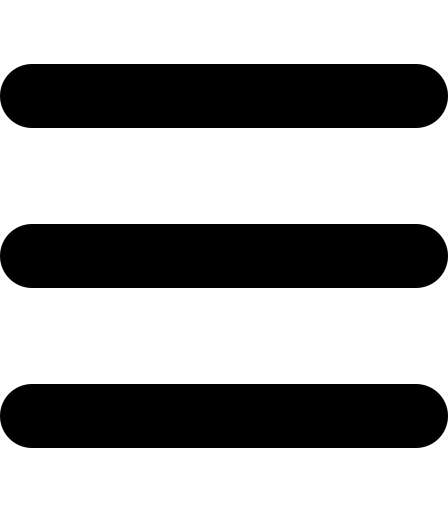
\includegraphics[width=0.2\textwidth]{imagenes/06_Diseno/bars-solid.png}}
\subfloat[Cámara]{
\label{subfig:camara_icon}
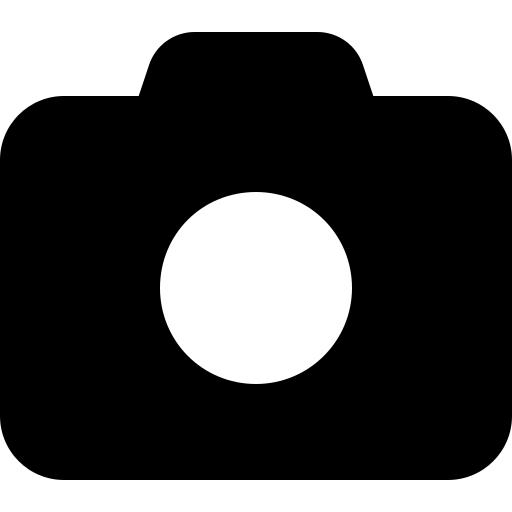
\includegraphics[width=0.2\textwidth]{imagenes/06_Diseno/camera-solid.png}}
\caption{Iconos usados en el sitio web}
\label{fig:iconos_vista}
\end{figure}

Todos los iconos de la Figura \ref{fig:iconos_vista} abstraen algún concepto de la página web. Por ejemplo, el icono de Telegram se coloca en un botón para deducir rápidamente que ese botón realiza alguna acción relacionada con la aplicación Telegram.

Otra parte del diseño de la vista que influye en la sencillez del sitio web es el diseño que se haga de cada una de las secciones de la página web. Dado que con el sitemap se consigue un diseño demasiado abstracto, también es útil elaborar los bocetos web o wireframes. Estos bocetos consisten en una representación visual de un sencillo esquema de la página web. En este caso se han realizado los bocetos de las siguientes secciones:

\begin{itemize}
\item \textbf{Página principal}: Está compuesta por una breve descripción del evento que aloja la actividad del chatbot de nuestro sistema, y la zona de actividades, donde se recomienda una serie de actividades (Figura \ref{fig:wireframe_pag_principal}).

\item \textbf{Actividad del chatbot}: En esta sección, al igual que pasa en la página principal, se visualiza una breve descripción; pero en este caso esta descripción es sobre la actividad del chatbot. Y además, se muestran los distintos accesos al chatbot a través de los distintos canales disponibles (Figura \ref{fig:wireframe_act_chatbot}).

\item \textbf{Captura de imágenes}: Dentro de esta sección volvemos a tener dos secciones, ya que para la gestión de las imágenes se debe tomar la imagen y posteriormente enviar la imagen para la deducción de la edad. En primer lugar, en la sección de captura de la imagen se muestra una ventana que irá mostrando el vídeo captado por la cámara y también se muestra un botón para realizar la captura. Y en segundo punto, en la sección de envío de la imagen se muestra una ventana que muestra la imagen tomada y también se muestra un botón para efectuar el envío (Figura \ref{fig:wireframe_capt_img}).

\item \textbf{Interfaz web}: Esta sección es simple, ya que sigue el diseño típico de un chat. Teniendo una entrada de texto y un visor de la conversación, donde aparecen los mensajes encapsulados orientados a la derecha o a la izquierda dependiendo del emisor del mensaje (Figura \ref{fig:wireframe_interfaz_web}).

\item \textbf{Interfaz de Telegram}: Esta sección es similar a la sección de la interfaz web, pero adaptado al diseño que tiene la aplicación de Telegram. Esta interfaz no deja de ser un chat de Telegram (Figura \ref{fig:wireframe_interfaz_telegram}).
\end{itemize}



\begin{figure}
    \centering
    \subfloat[Wireframe de la página principal]{
    \begin{subfigure}
        \centering
        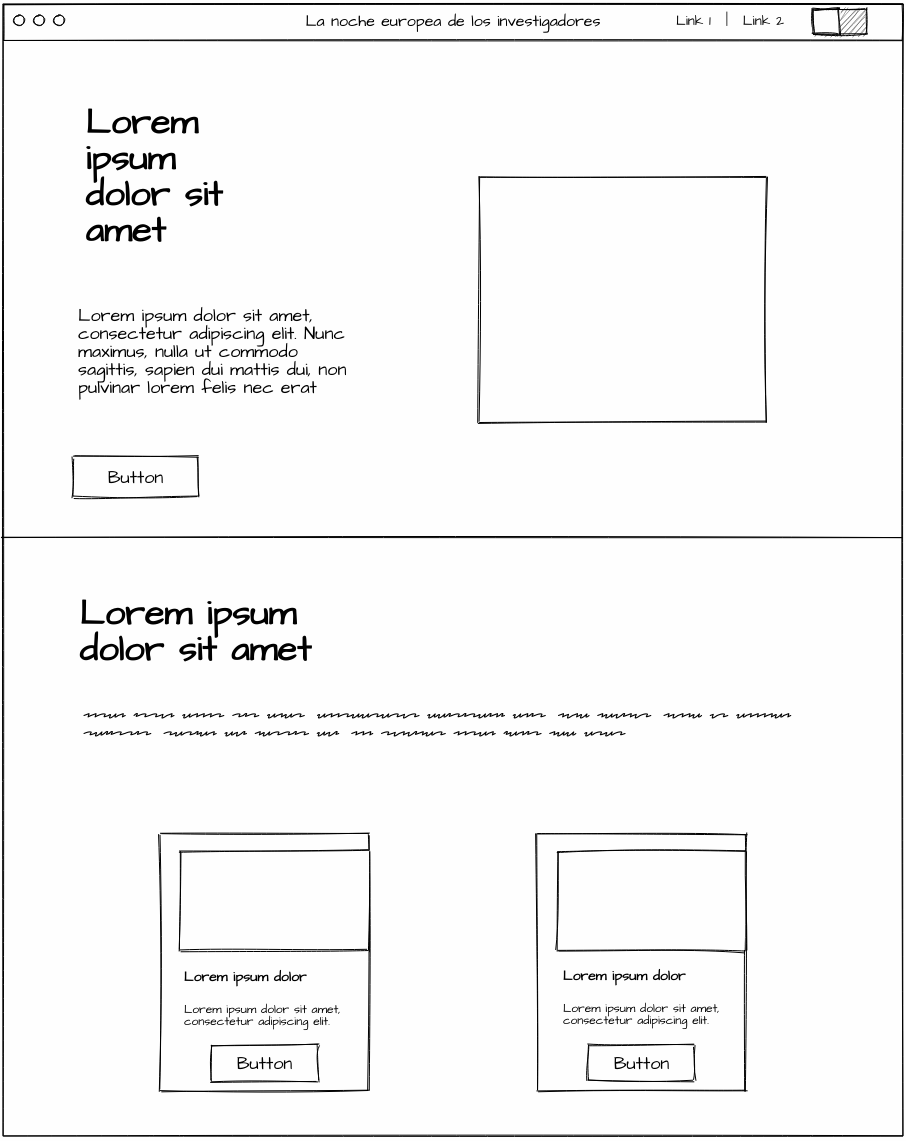
\includegraphics[width=0.5\textwidth]{imagenes/06_Diseno/pagina_principal.png}
        \label{fig:wireframe_pag_principal}
    \end{subfigure}
    }
    \subfloat[Wireframe de la actividad del chatbot]{
    \begin{subfigure}
        \centering
        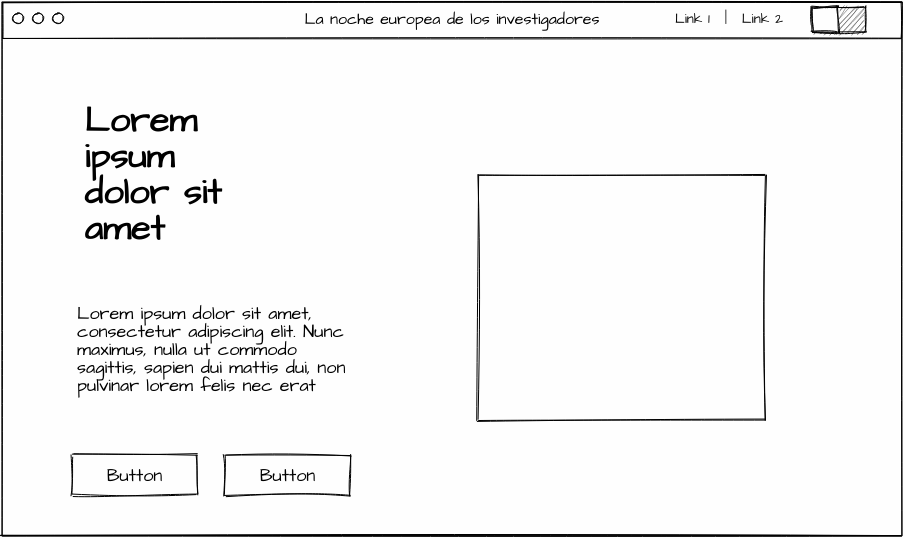
\includegraphics[width=0.5\textwidth]{imagenes/06_Diseno/actividad_chatbot.png}
        \label{fig:wireframe_act_chatbot}
    \end{subfigure}
    }
    \hfill
    \subfloat[Wireframe de la captura de imágenes]{
    \begin{subfigure}
        \centering
        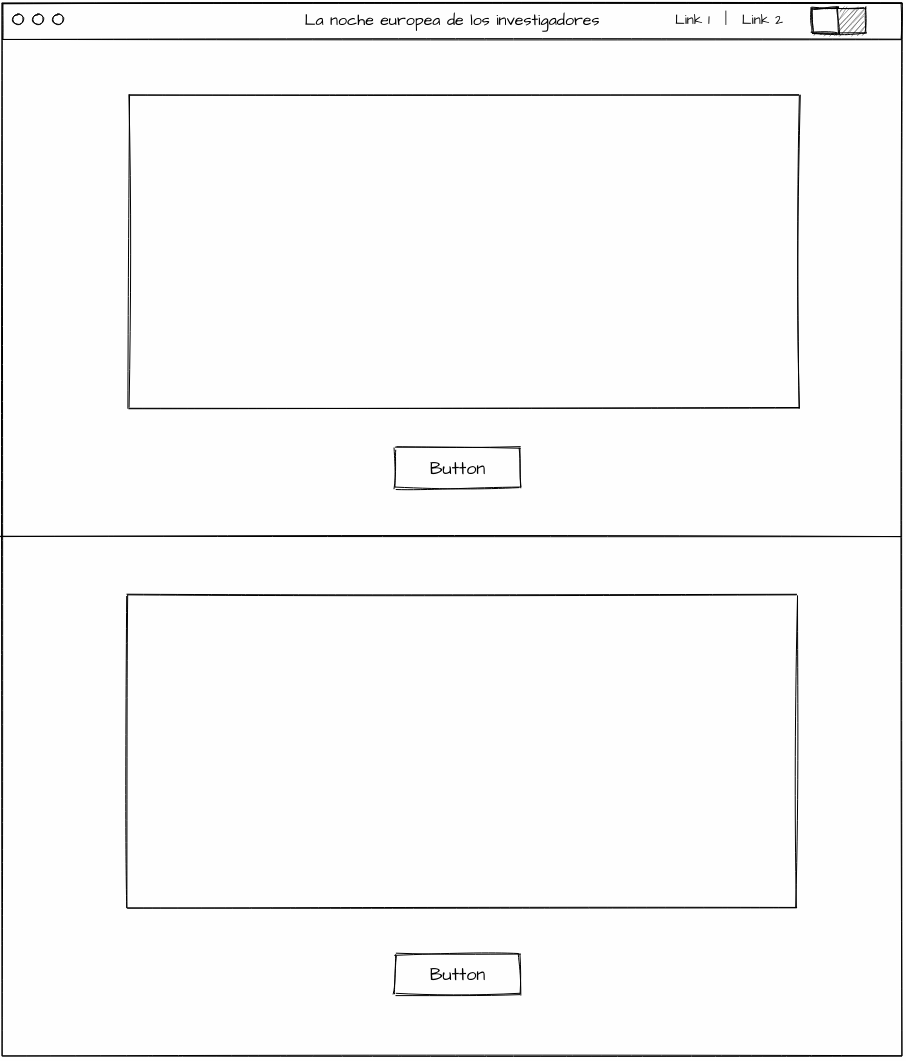
\includegraphics[width=0.5\textwidth]{imagenes/06_Diseno/capturar_imagen.png}
        \label{fig:wireframe_capt_img}
    \end{subfigure}
    }
    \subfloat[Wireframe de la interfaz web]{
    \begin{subfigure}
        \centering
        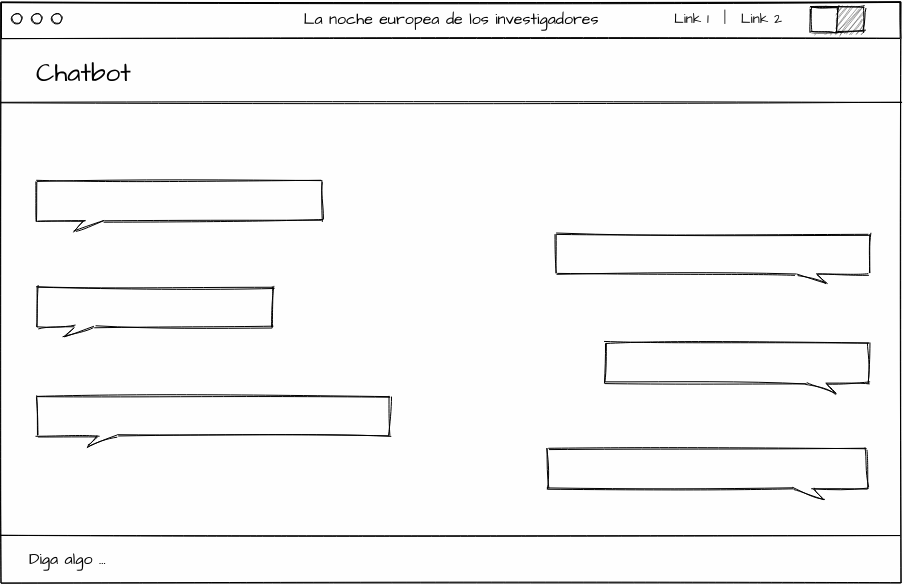
\includegraphics[width=0.5\textwidth]{imagenes/06_Diseno/interfaz_web.png}
        \label{fig:wireframe_interfaz_web}
    \end{subfigure}
    }
    \hfill
    \subfloat[Wireframe de la interfaz de Telegram]{
    \begin{subfigure}
        \centering
        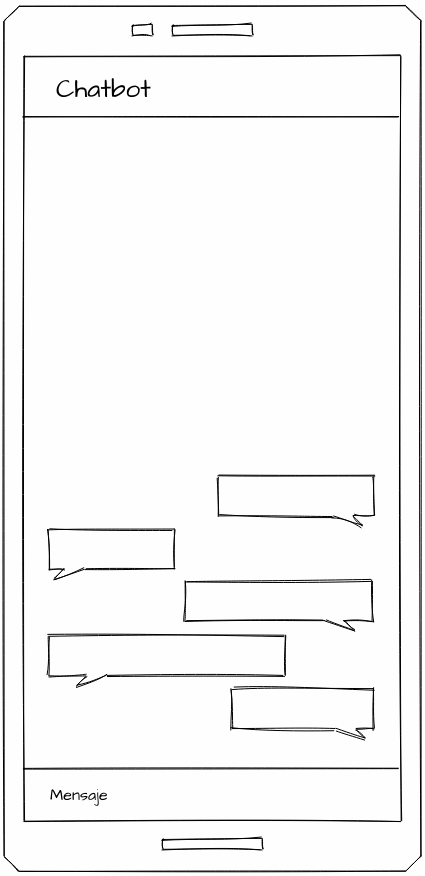
\includegraphics[width=0.2\textwidth]{imagenes/06_Diseno/interfaz_telegram.png}
        \label{fig:wireframe_interfaz_telegram}
    \end{subfigure}
    }
\caption{Wireframes de la Vista}
\label{fig:wireframes_vista}
\end{figure}




Todas las secciones descritas tienen en común las barras de navegación, tanto la que se encuentra en la parte superior de la página web como la lateral. Estas barras de navegación estarán compuestas por el logo del evento, una serie de \glspl{link} para el rápido movimiento a través del sitio web, un interruptor para el cambio de tema de colores, y un botón para desplegar menú lateral si es necesario según el dispositivo que se esté utilizando.

Llegados a este punto tenemos un claro diseño de los elementos que componen el sitio web; aunque, por otra parte, otro objetivo que influye en el diseño de la vista es la obtención de una interfaz armónica (Tabla \ref{tab:HU3}), es decir, una interfaz que tiene colores llamativos para el usuario, pero que no llega a cansarlo rápidamente. Para la elección de colores me he basado en un principio en los colores empleados en la página oficial del evento de La Noche Europea de l@s Investigador@s \footnote{\url{https://lanochedelosinvestigadores.fundaciondescubre.es}}. Los colores que he elegido son más claros de los elegidos para la página oficial. Estos colores van desde el azul al blanco. Y en concreto para la tipografía, el negro y el dorado en ciertas ocasiones. Pero los colores anteriormente descritos forman parte del modo claro de la página web. Como se ha comentado en anteriores párrafos de este apartado, cada página web dispone de un interruptor para el cambio al modo oscuro. La utilización de dos modos de colores, uno claro y otro oscuro; está muy extendida actualmente dada la gran acogida del modo oscuro en muchas aplicaciones con gran volumen de usuarios. En la elección para los colores del modo oscuro se debe tener en cuenta que el texto debe seguir siendo legible, para ello se deben elegir colores que tenga mucho contraste entre ellos. Los colores utilizados para nuestro modo oscuro van desde el gris al negro, y en algunas ocasiones el naranja. Y en concreto, para la tipografía, el blanco, el gris en ciertos textos secundarios, y el dorado en ciertas ocasiones.

\section{Diseño del Controlador}

El Controlador deberá ser la unión entre la Vista y el Modelo. Por esta razón, deberá tener entradas que gestionen las peticiones creadas por la Vista, las procesen y las reenvíen al Modelo; y entradas que gestionen las peticiones creadas por el Modelo, como respuesta a las peticiones llegadas desde la Vista, las procesen y las reenvíen a la Vista.

Este Controlador será un servidor que tendrá al menos las entradas necesarias para gestionar las distintas secciones del sitio web, cuyo diseño se expuso en el apartado de diseño de la Vista (Apartado \ref{sec:diseño_vista}). Estas secciones son las siguientes:

\begin{itemize}
\item Página principal
\item Actividad de chatbot
\item Captura de imágenes
\item Interfaz web para adultos
\item Interfaz web para niños
\end{itemize}

Las únicas secciones del sitio web que no tendrán una sección en el servidor son las interfaces de Telegram, ya que son gestionadas por la propia aplicación de Telegram. Parte de estas secciones no requerirán una interacción con el Modelo; mientras que otras si lo requerirán, como puede ser la sección de captura de imágenes.

Para tener una visión más abstracta de todo el proceso seguido a través del sitio web hasta llegar a la interfaz del chatbot, se ha elaborado un diagrama de actividad, el cual se puede ver en la Figura \ref{fig:diagram_acti_sitio_web}.

\begin{figure}[h]
\centering
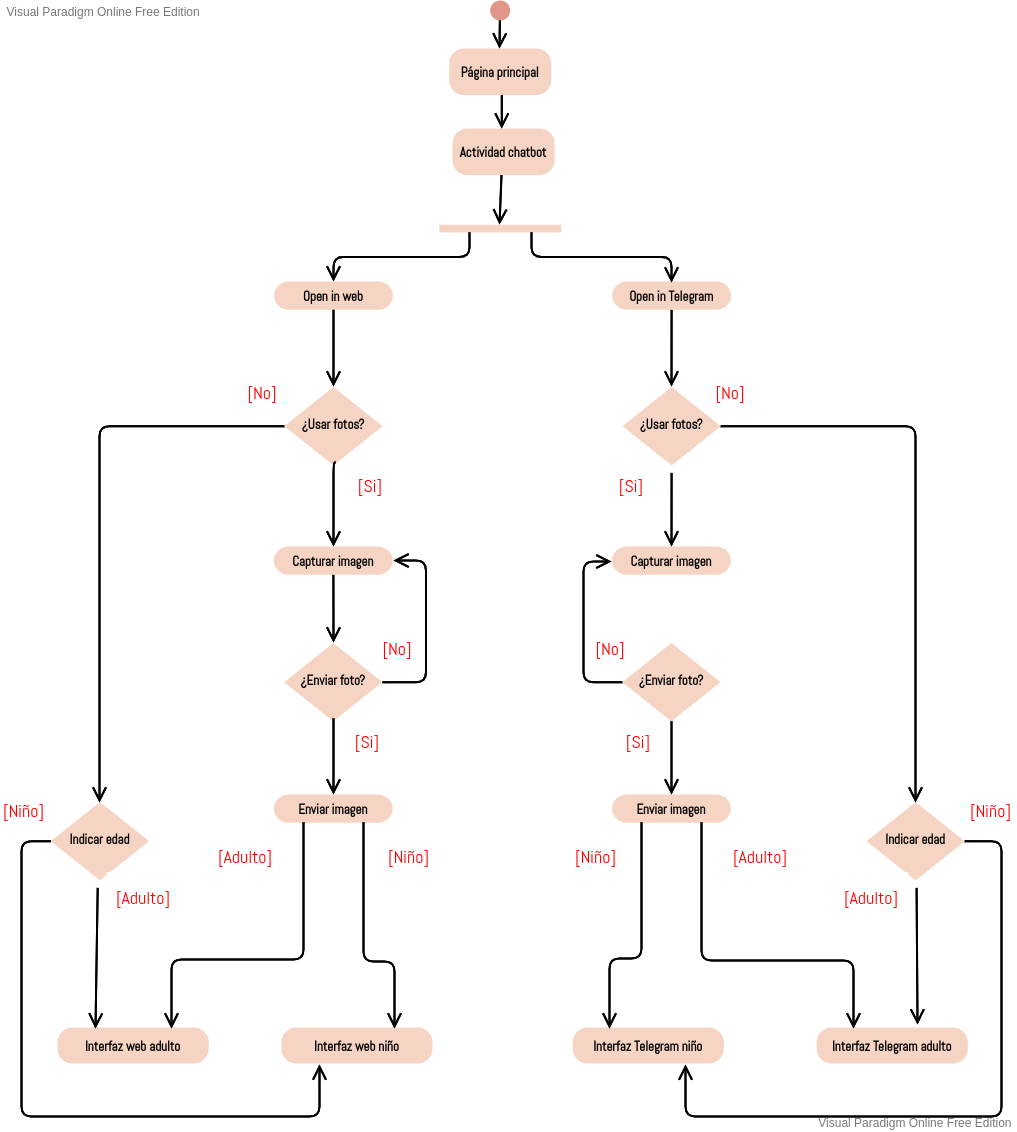
\includegraphics[width=0.7\textwidth]{imagenes/06_Diseno/diagram_acti_sitio_web.png}
\caption{Diagrama de actividad del acceso a la interfaz del chatbot}
\label{fig:diagram_acti_sitio_web}
\end{figure}

En la Figura \ref{fig:diagram_acti_sitio_web} se pueden ver todas los puntos de decisión que tiene el usuario a lo largo de su interacción con el sitio web, y cuáles son los posibles caminos existentes para llegar a alguna de las interfaces del chatbot.

Aparte de todas las secciones mencionadas, el servidor contará con otras secciones que serán definidas en la implementación, ya que serán necesarias por las condiciones impuestas por las distintas herramientas que se usen a la hora de implementar el Controlador.

Aparte de indicar el diseño de las secciones del sitio web, es interesante tener una primera imagen de como deben quedar dos de las secciones más importantes del sistema, las cuales son llevadas a cabo por el Controlador. La primera es la gestión de la conversación, la cual se puede ver en la Figura \ref{fig:diagram_acti_make_conver}. Y la segunda es la gestión del procesado de la imagen, la cual se puede ver en la Figura \ref{fig:diagram_acti_proce_imagen}.

\begin{figure}[h]
\centering
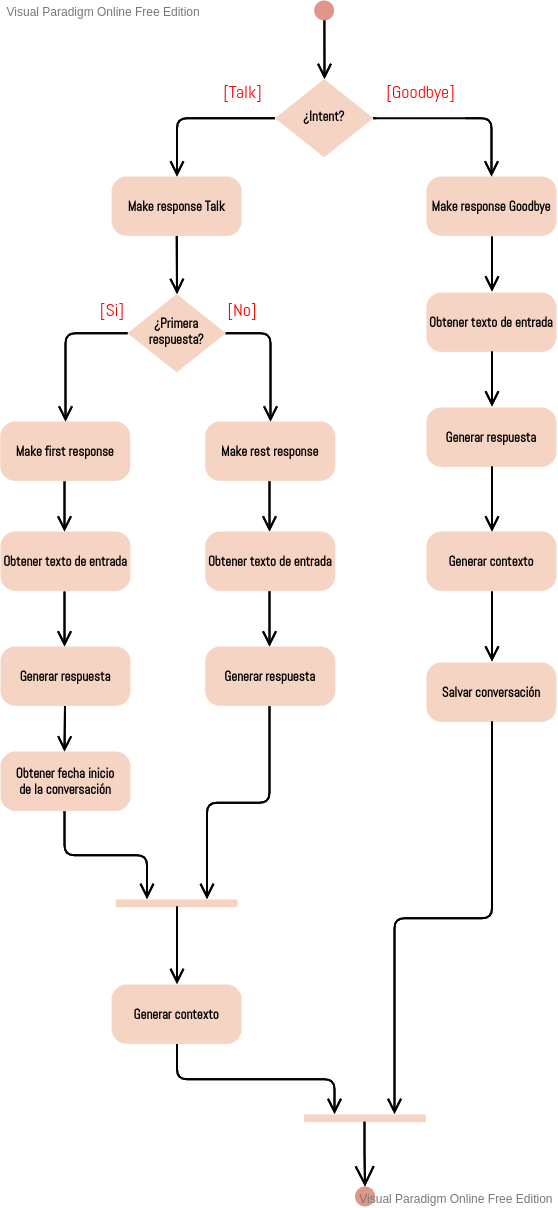
\includegraphics[width=0.4\textwidth]{imagenes/06_Diseno/diagram_acti_make_conver.png}
\caption{Diagrama de actividad de la gestión de la conversación}
\label{fig:diagram_acti_make_conver}
\end{figure}

\begin{figure}[h]
\centering
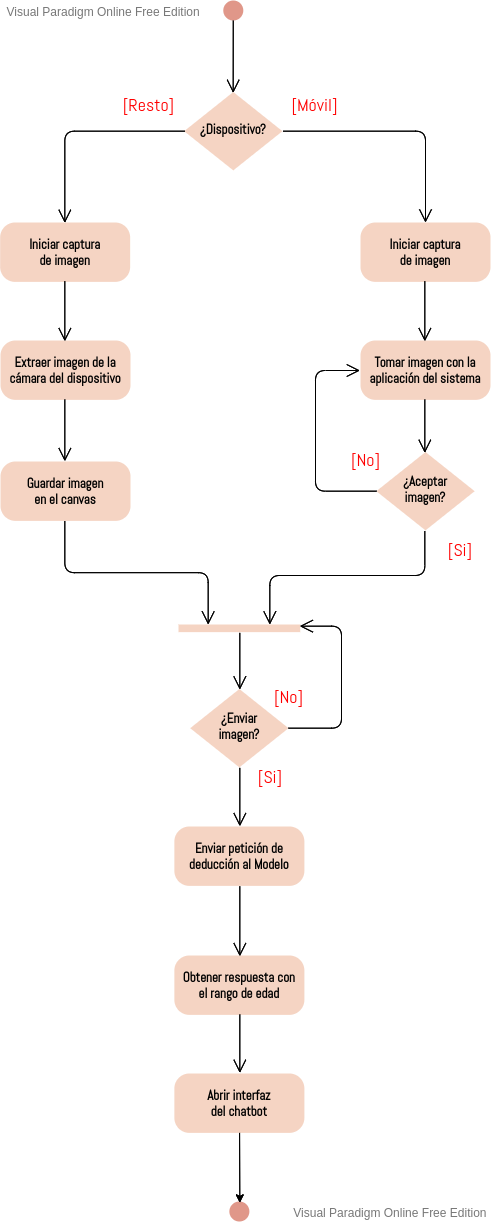
\includegraphics[width=0.4\textwidth]{imagenes/06_Diseno/diagram_acti_proce_imagen.png}
\caption{Diagrama de actividad de la gestión del procesado de la imagen}
\label{fig:diagram_acti_proce_imagen}
\end{figure}

\section{Diseño del Modelo}

El diseño del Modelo de nuestro sistema se divide en varias partes debido a que este Modelo suministra distintos datos al Controlador dependiendo de la parte del Modelo que se utilice.

Algo a destacar es que para implementar todas las funcionalidades del Modelo del sistema se han empleado modelos basados en \gls{Transformers} basados en \gls{Transformers} implementados en \gls{PyTorch}.

\subsection*{Módulo de generación de respuestas}

Esta parte del Modelo es la encargada de proporcionar las respuestas a las entradas proporcionadas por el Controlador. Siguiendo la filosofía del Transfer Learning, la cual fue explicada en el análisis del estado del arte (Apartado \ref{sec:analisis_estado_arte}), para la generación de respuestas se va a hacer uso de modelos pre entrenados del modelo BlenderBot. De esta forma facilitamos la creación de un chatbot orientado a la funcionalidad que buscamos.

\subsection*{Módulo de deducción de edad}

De igual forma que se pretende hacer con el modelo generador de respuestas, para el módulo de deducción de edad se hará empleo de modelos pre entrenados para el reconocimiento de imágenes.

\subsection*{Log de las conversaciones}

Los datos a guardar en este log serán las conversaciones terminadas con los distintos usuarios del sistema. El diseño para modelar estas conversaciones en el log estará compuesto por una única tabla. Los elementos de esta tabla serán los siguientes:

\begin{itemize}
\item Contenido de la conversación
\item Fecha de inicio de la conversación
\item Fecha de finalización de la conversación
\item Duración de la conversación
\item Edad del usuario con el que se realizó la conversación
\item Identificador de la conversación
\item Verificación de la conversación por parte del administrado del sistema
\end{itemize}

Cabe destacar que el identificador de la conversación será la clave principal de la tabla, la duración de la conversación será un atributo calculado a partir de la fecha de inicio y de finalización, y por último, el contenido de la conversación estará compuesto por la sucesión de entradas y de respuestas que ha recibido el sistema, indicando tanto las entradas como las respuestas en español y en inglés.

\subsection*{Entrenamiento de modelos}

A pesar de que utilicemos modelos pre entrenados, los cuales puedan funcionar desde el primer momento, debemos acercar el dominio de los modelos a la funcionalidad que queremos que tengan. Para realizar este cambio de dominio se debe realizar un ajuste (fine-tuning) de los modelos pre entrenados. Se hace un ajuste y no un entrenamiento desde cero por la simple razón de que estamos usando modelo pre entrenados y queremos aprovecharnos del entrenamiento que llevan implícito estos modelos. El ajuste de los modelos requerirá de unos conjuntos de datos. Estos conjuntos de datos serán los que modifiquen el dominio del modelo, por lo tanto, los conjuntos de datos deberán representar el nuevo dominio que queremos que tengan los modelos. El ajuste, a diferencia de un entrenamiento desde cero, consiste en la ejecución de un entrenamiento de unas pocas épocas de duración. Se efectúa este breve entrenamiento porque queremos adaptar ligeramente el dominio, ya que un movimiento muy brusco provocaría la pérdida del trabajo implícito que traen los modelos pre entrenados. Si necesitamos adaptar mucho el dominio, sería más recomendable buscar otro modelo pre entrenado o entrenar uno propio desde cero.

\subsection*{Generación de los conjuntos de datos}

Por supuesto estos conjuntos de datos no vienen elaborados por defecto, debemos generar nuestros propios conjuntos de datos a base de extraer información de distintas fuentes. Deberemos generar los conjuntos de datos con un formato adecuado para su uso en el ajuste de los modelos. Esta parte es la más difícil de llevar a cabo entre todas las partes necesarias para elaborar un chatbot propio, dada la complejidad de encontrar información sobre algunos temas. Todo dependerá de la funcionalidad que queramos que tenga el chatbot, y de la facilidad que encontremos a la hora de extraer información útil.

